\documentclass[a4paper]{article}
\usepackage{cmap}
\usepackage{mathtext}
\usepackage{amssymb}
\usepackage{amsmath}
\usepackage[russian]{babel}
\usepackage{indentfirst}
\usepackage[pdftex]{graphicx}
\usepackage{multirow}
\usepackage{mathrsfs}
\usepackage{biblatex}
\usepackage{siunitx}
\usepackage[left=2cm,right=2cm,top=2cm,bottom=2cm]{geometry}
\usepackage{fancyhdr}
\bibliography{bib}
\pagestyle{fancy}
\newcommand{\const}{\mathrm{const}}
\newcommand{\rref}[1]{(\ref{#1})}
\newenvironment{comment}{}{}
\newcommand{\picref}[1]{рис. \ref{#1}}
\newcommand{\mbf}{\mathbf}
\newcommand{\Equip}[3]{
	
	{\bf #1:} $\Delta = \pm #2\; #3$}
\newcommand{\equip}[1]{
	
	{\bf #1}}
\newcommand{\labname}{Эффект Франка--Герца} 	% название пиши здесь
\newcommand{\labnum}{5.2.1}		% номер вводи здесь
\fancyfoot{}
\fancyhead[RE, RO]{\thepage}
\fancyhead[LE, LO]{Лабораторная работа \labnum \space \labname}
\title{Лабораторная работа \labnum \space \labname} % Название работы здесь
\author{Иван Сладков}
\begin{document}
\maketitle
\thispagestyle{empty}
\section{Аннотация}
В данной работе проводится измерение энергии первого уровня атома гелия методом электронного возбуждения в динамическом и статическом режимах.

\section{Теоретические сведения}

Разреженный одноатомный газ (в нашем случае -- гелий) заполняет трёхэлектродную лампу. Электроны, испускаемые разогретым катодом, ускоряются в постоянном электрическом поле, созданным между катодом и сетчатым анодом лампы. Передвигаясь от катода к аноду, электроны сталкиваются с атомами гелия. Если энергия электрона, налетающего на атом, недостаточна для того, чтобы перевести его в возбуждённое состояние (или ионизовать), то возможны только упругие соударения, при которых электроны почти не теряют энергии, так как их масса в тысячи раз меньше массы атомов.


По мере увеличения разности потенциалов между анодом и катодом энергия электронов увеличивается и, в конце концов, оказывается достаточной для возбуждения атомов. При таких -- неупругих -- столкновениях кинетическая энергия налетающего электрона передаётся одному из атомных электронов, вызывая его переход на свободный энергетический уровень (возбуждение) или совсем отрывая его от атома (ионизация).

При увеличении потенциала анода ток в лампе вначале растёт, подобно тому как это происходит в вакуумном диоде (рис. 2). Однако, когда энергия электронов становится достаточной для возбуждения атомов, ток коллектора резко уменьшается. Это происходит потому, что при неупругих соударениях с атомами электроны почти полностью теряют свою энергию и не могут преодолеть задерживающего потенциала между анодом и коллектором. При дальнейшем увеличении потенциала анода ток коллектора вновь возрастает: электроны, испытавшие неупругие соударения, при дальнейшем движении к аноду успевают набрать энергию, достаточную для преодоления задерживающего потенциала.


\begin{figure}[tbh]
	\centering
	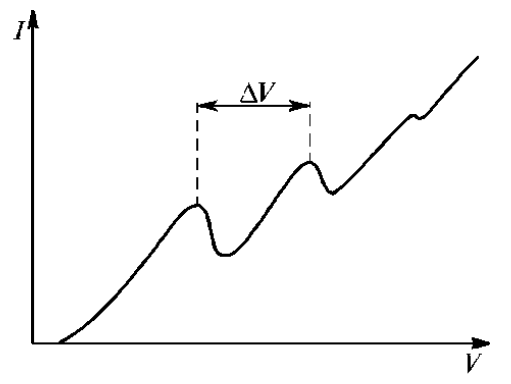
\includegraphics[width=0.4\textheight]{Screenshot_1}
	\caption{Характер зависимости $I (U)$}
	\label{fig:screenshot1}
\end{figure}

\subsection{Расчётные формулы}

Кинетическая энергия электрона 1 уровня равна:
\begin{equation}\label{key}
	E = \overline{e} \Delta V \left[эВ\right],
\end{equation}
где $ \Delta V $ -- разность между двумя пиками (см. рис. \ref{fig:screenshot1}).

\section{Оборудование и инструментальные погрешности}

Схема экспериментальной установки отображена на рис. \ref{fig:screenshot2} и \ref{fig:screenshot3}.

\begin{figure}[tbh]
	\centering
	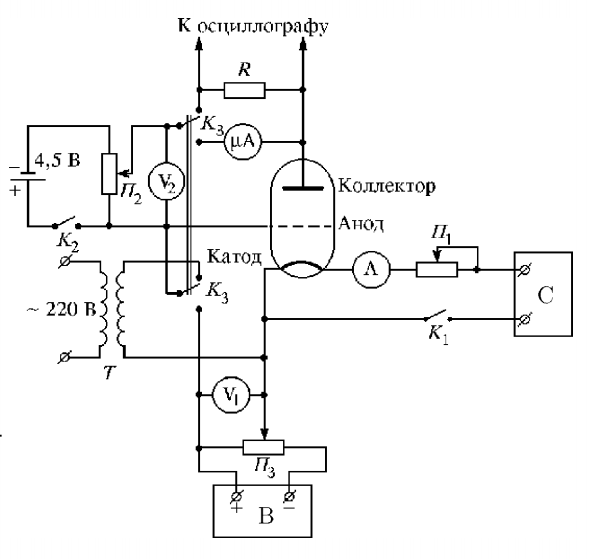
\includegraphics[height=0.4\textheight]{Screenshot_2}
	\caption{Принципиальная схема установки}
	\label{fig:screenshot2}
\end{figure}

\begin{figure}[tbh]
	\centering
	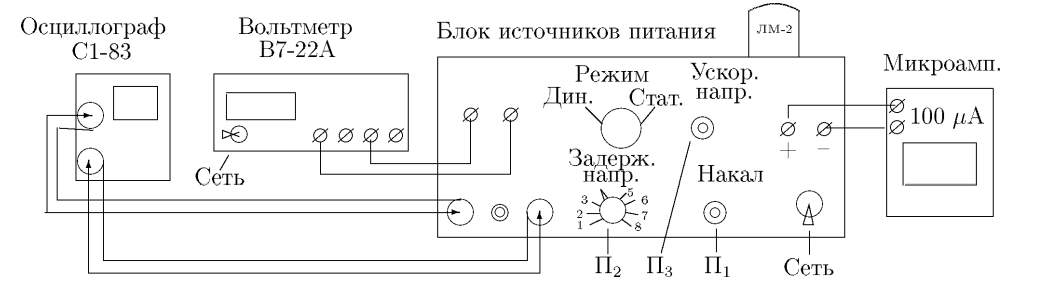
\includegraphics[width=0.6\textheight]{Screenshot_3}
	\caption{Блок-схема экспериментальной установки}
	\label{fig:screenshot3}
\end{figure}


В работе используются:

\Equip{Осциллограф}{0.4}{В} (в данном опыте)
\Equip{Вольтметр}{0.1}{В}
\Equip{Миллиамперметр}{0.5}{мА}
\equip{Блок источников питания}
\equip{Газонаполненная лампа} (гелий)

\section{Результаты измерений и обработка данных}

\subsection{Динамический метод}

По результатам, полученным на экране осциллографа (рис. \ref{fig:screenshot4}, \ref{fig:screenshot5}, \ref{fig:screenshot6}) получим данные табл. \ref{tab:1}.

 \begin{table}[h]
 	\centering
 	\begin{tabular}{|l|l|l|}
 		\hline
 		$V_з, \;В$ & $\Delta V, \; В$ & $E,\; эВ$ \\ \hline
 		4          & $15\pm 2$               & $15\pm 2$        \\ \hline
 		6          & $18\pm 2$               & $18\pm 2$        \\ \hline
 		8          & $18\pm 2$               & $18\pm 2$        \\ \hline
 	\end{tabular}
 \label{tab:1}
 \caption{Результаты динамического измерения}
 \end{table}

По итогу,
\begin{equation}\label{key}
	E \approx 17 \pm 3 \; эВ.
\end{equation}

\begin{figure}[tbh]
	\centering
	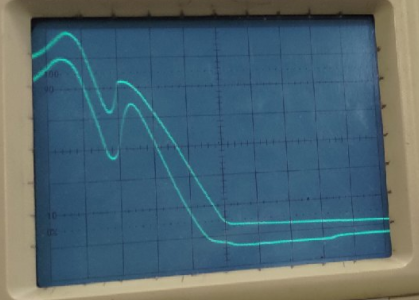
\includegraphics[width=0.7\linewidth]{Screenshot_4}
	\caption{Результат для $V_з = 4 \;В$}
	\label{fig:screenshot4}
\end{figure}

\begin{figure}[tbh]
	\centering
	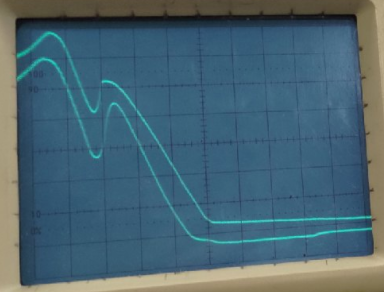
\includegraphics[width=0.7\linewidth]{Screenshot_5}
	\caption{Результат для $V_з = 6\; В$}
	\label{fig:screenshot5}
\end{figure}

\begin{figure}[tbh]
	\centering
	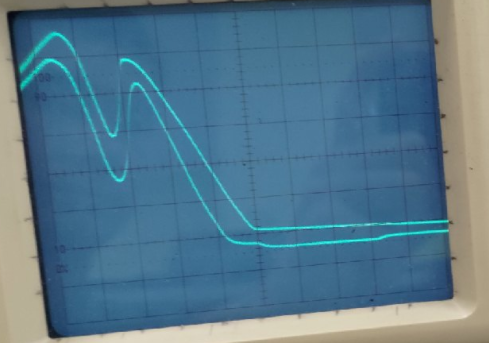
\includegraphics[width=0.7\linewidth]{Screenshot_6}
	\caption{Результат для $V_з = 8\; В$}
	\label{fig:screenshot6}
\end{figure}

\subsection{Статический метод}

Полученные статическим методом результаты отобразим на графиках. По 1 и 2 графику невозможно судить о положении максимумов, но 3 график позволяет их найти. Учтём как минимум, так и максимум.

\begin{table}[h]
	\centering
	\begin{tabular}{|l|l|l|}
		\hline
		$V_з, \;В$ & $\Delta V, \; В$ & $E,\; эВ$ \\ \hline
		8          & 23.9             & 23.9        \\ \hline
		8          & 16.4             & 16.4      \\ \hline
	\end{tabular}
	\caption{Результат измерения статическим методом}
	\label{tab:my-table}
\end{table}

\begin{equation}\label{key}
	E\approx 20\pm 5 \; эВ.
\end{equation}

\begin{figure}[tbh]
	\centering
	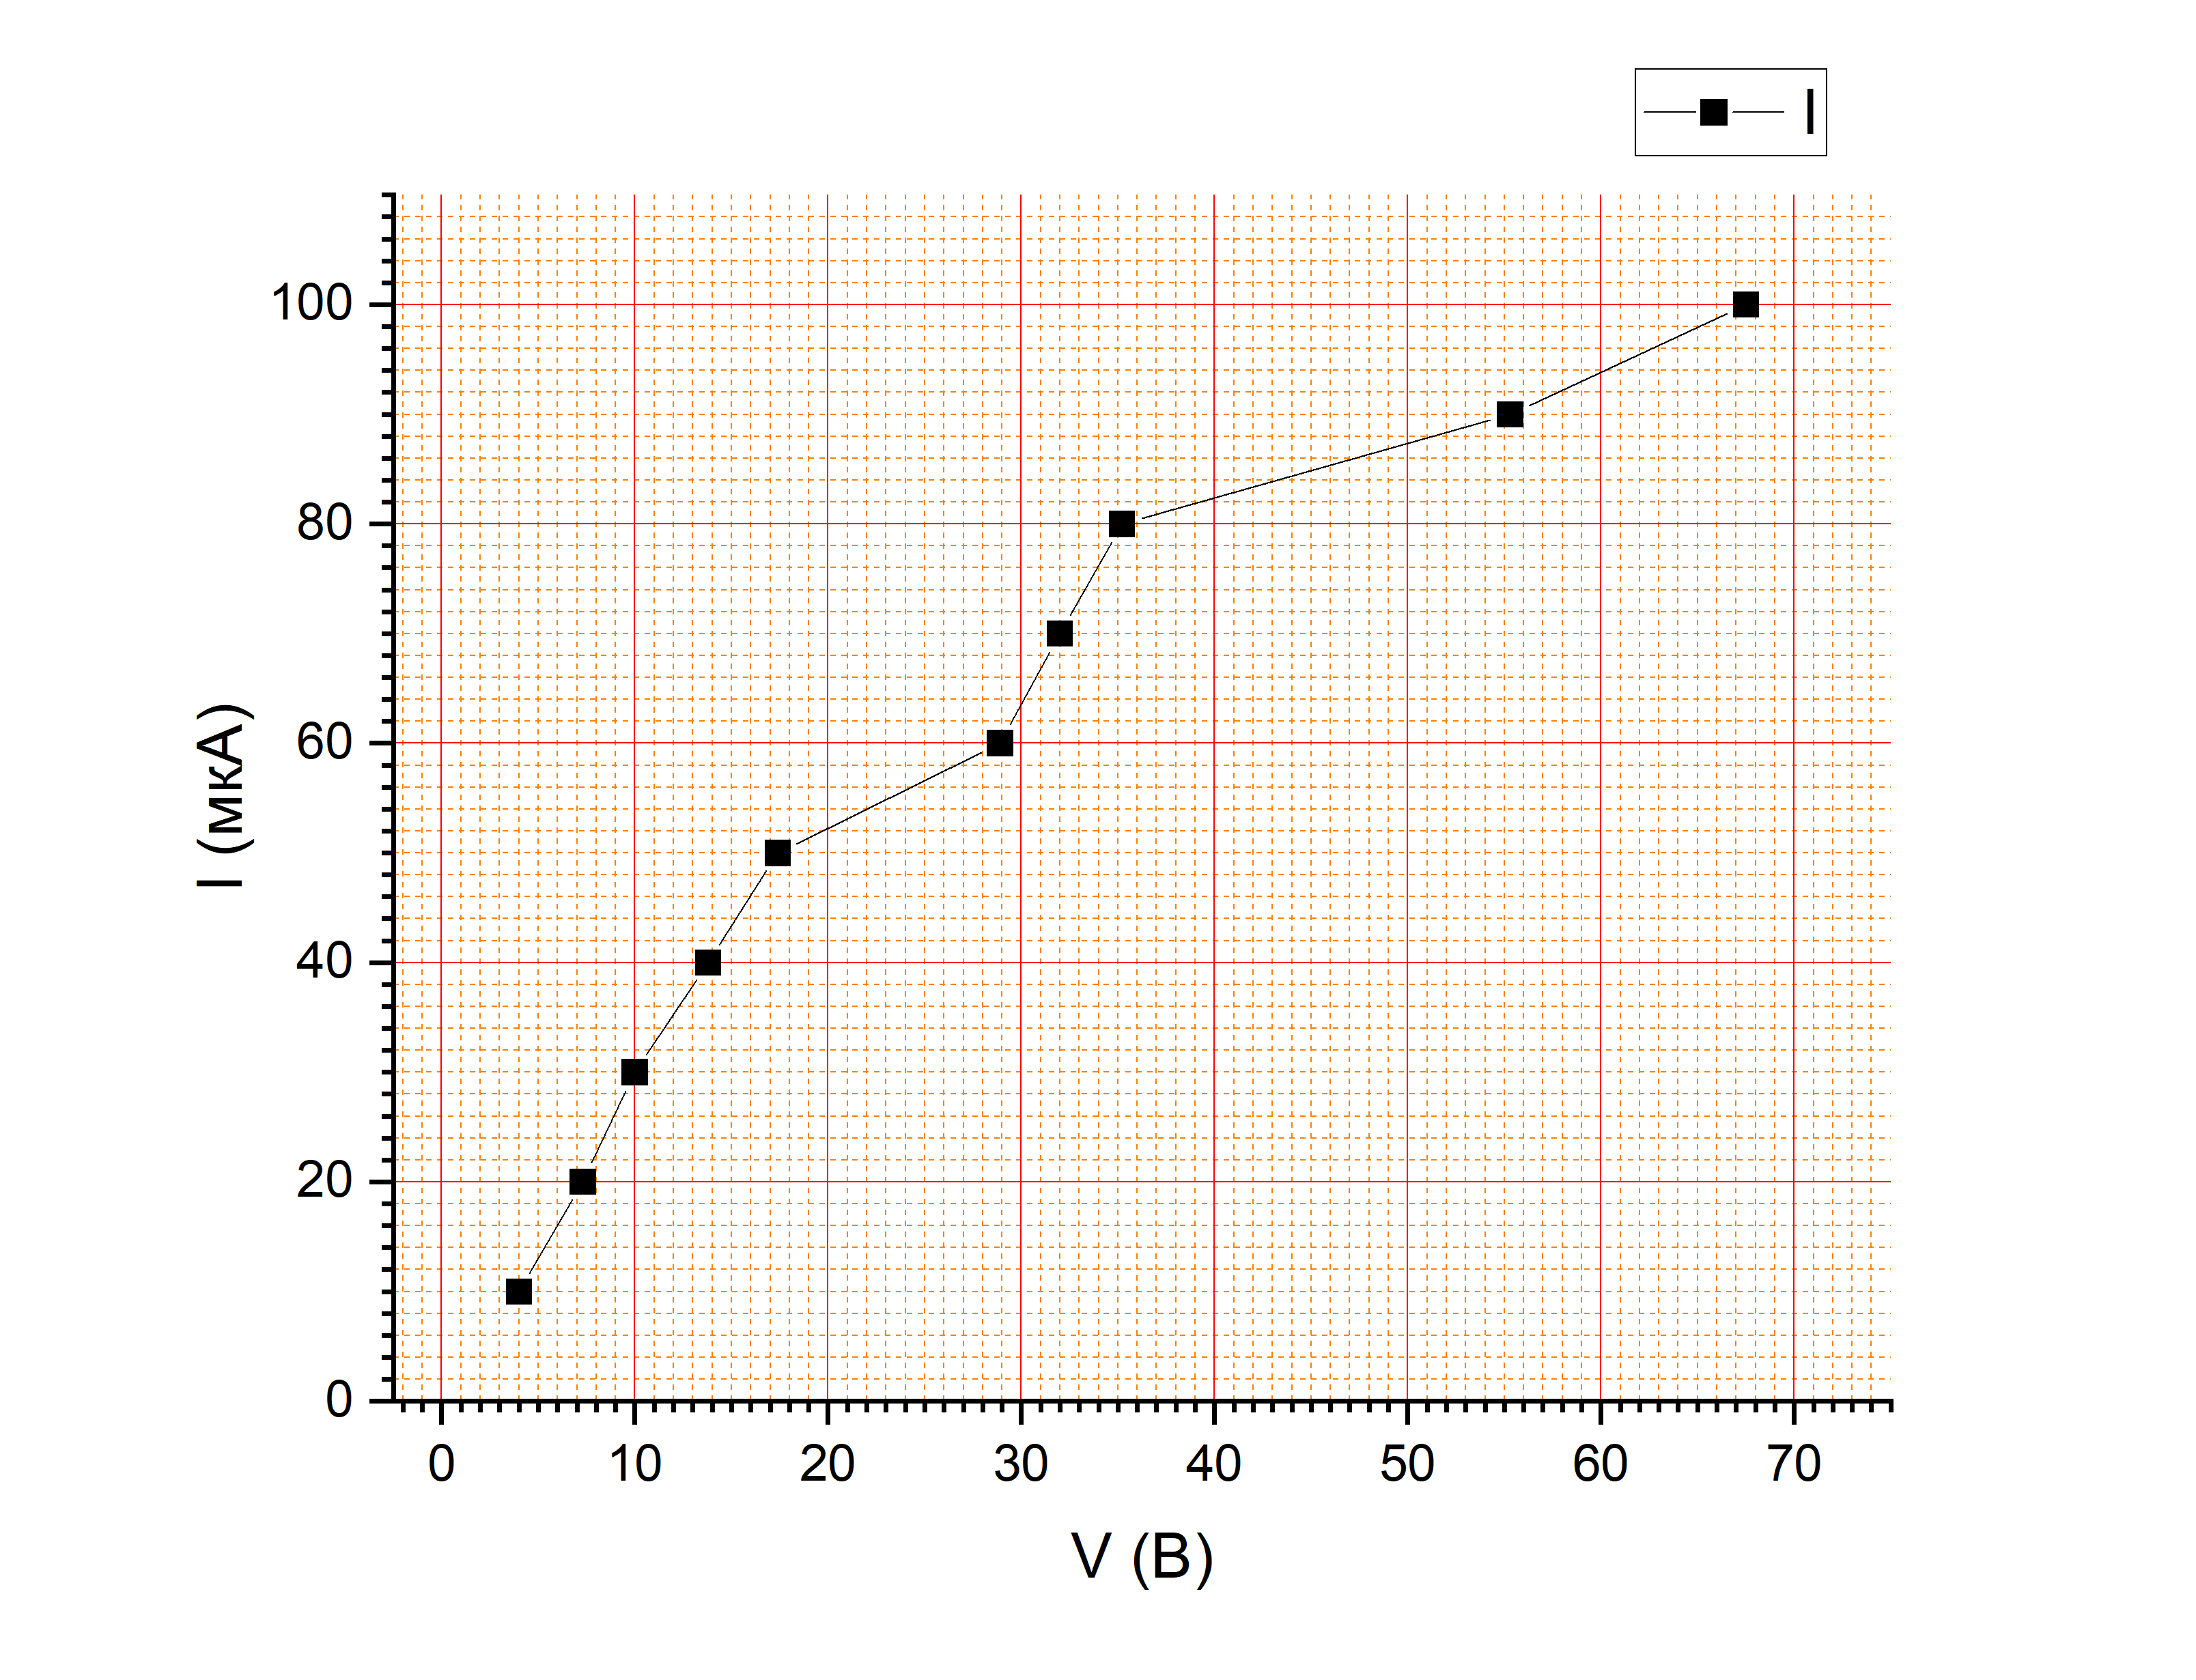
\includegraphics[width=0.7\linewidth]{Graph1}
	\caption{$V_з = 4 \;В$}
	\label{fig:graph1}
\end{figure}

\begin{figure}[tbh]
	\centering
	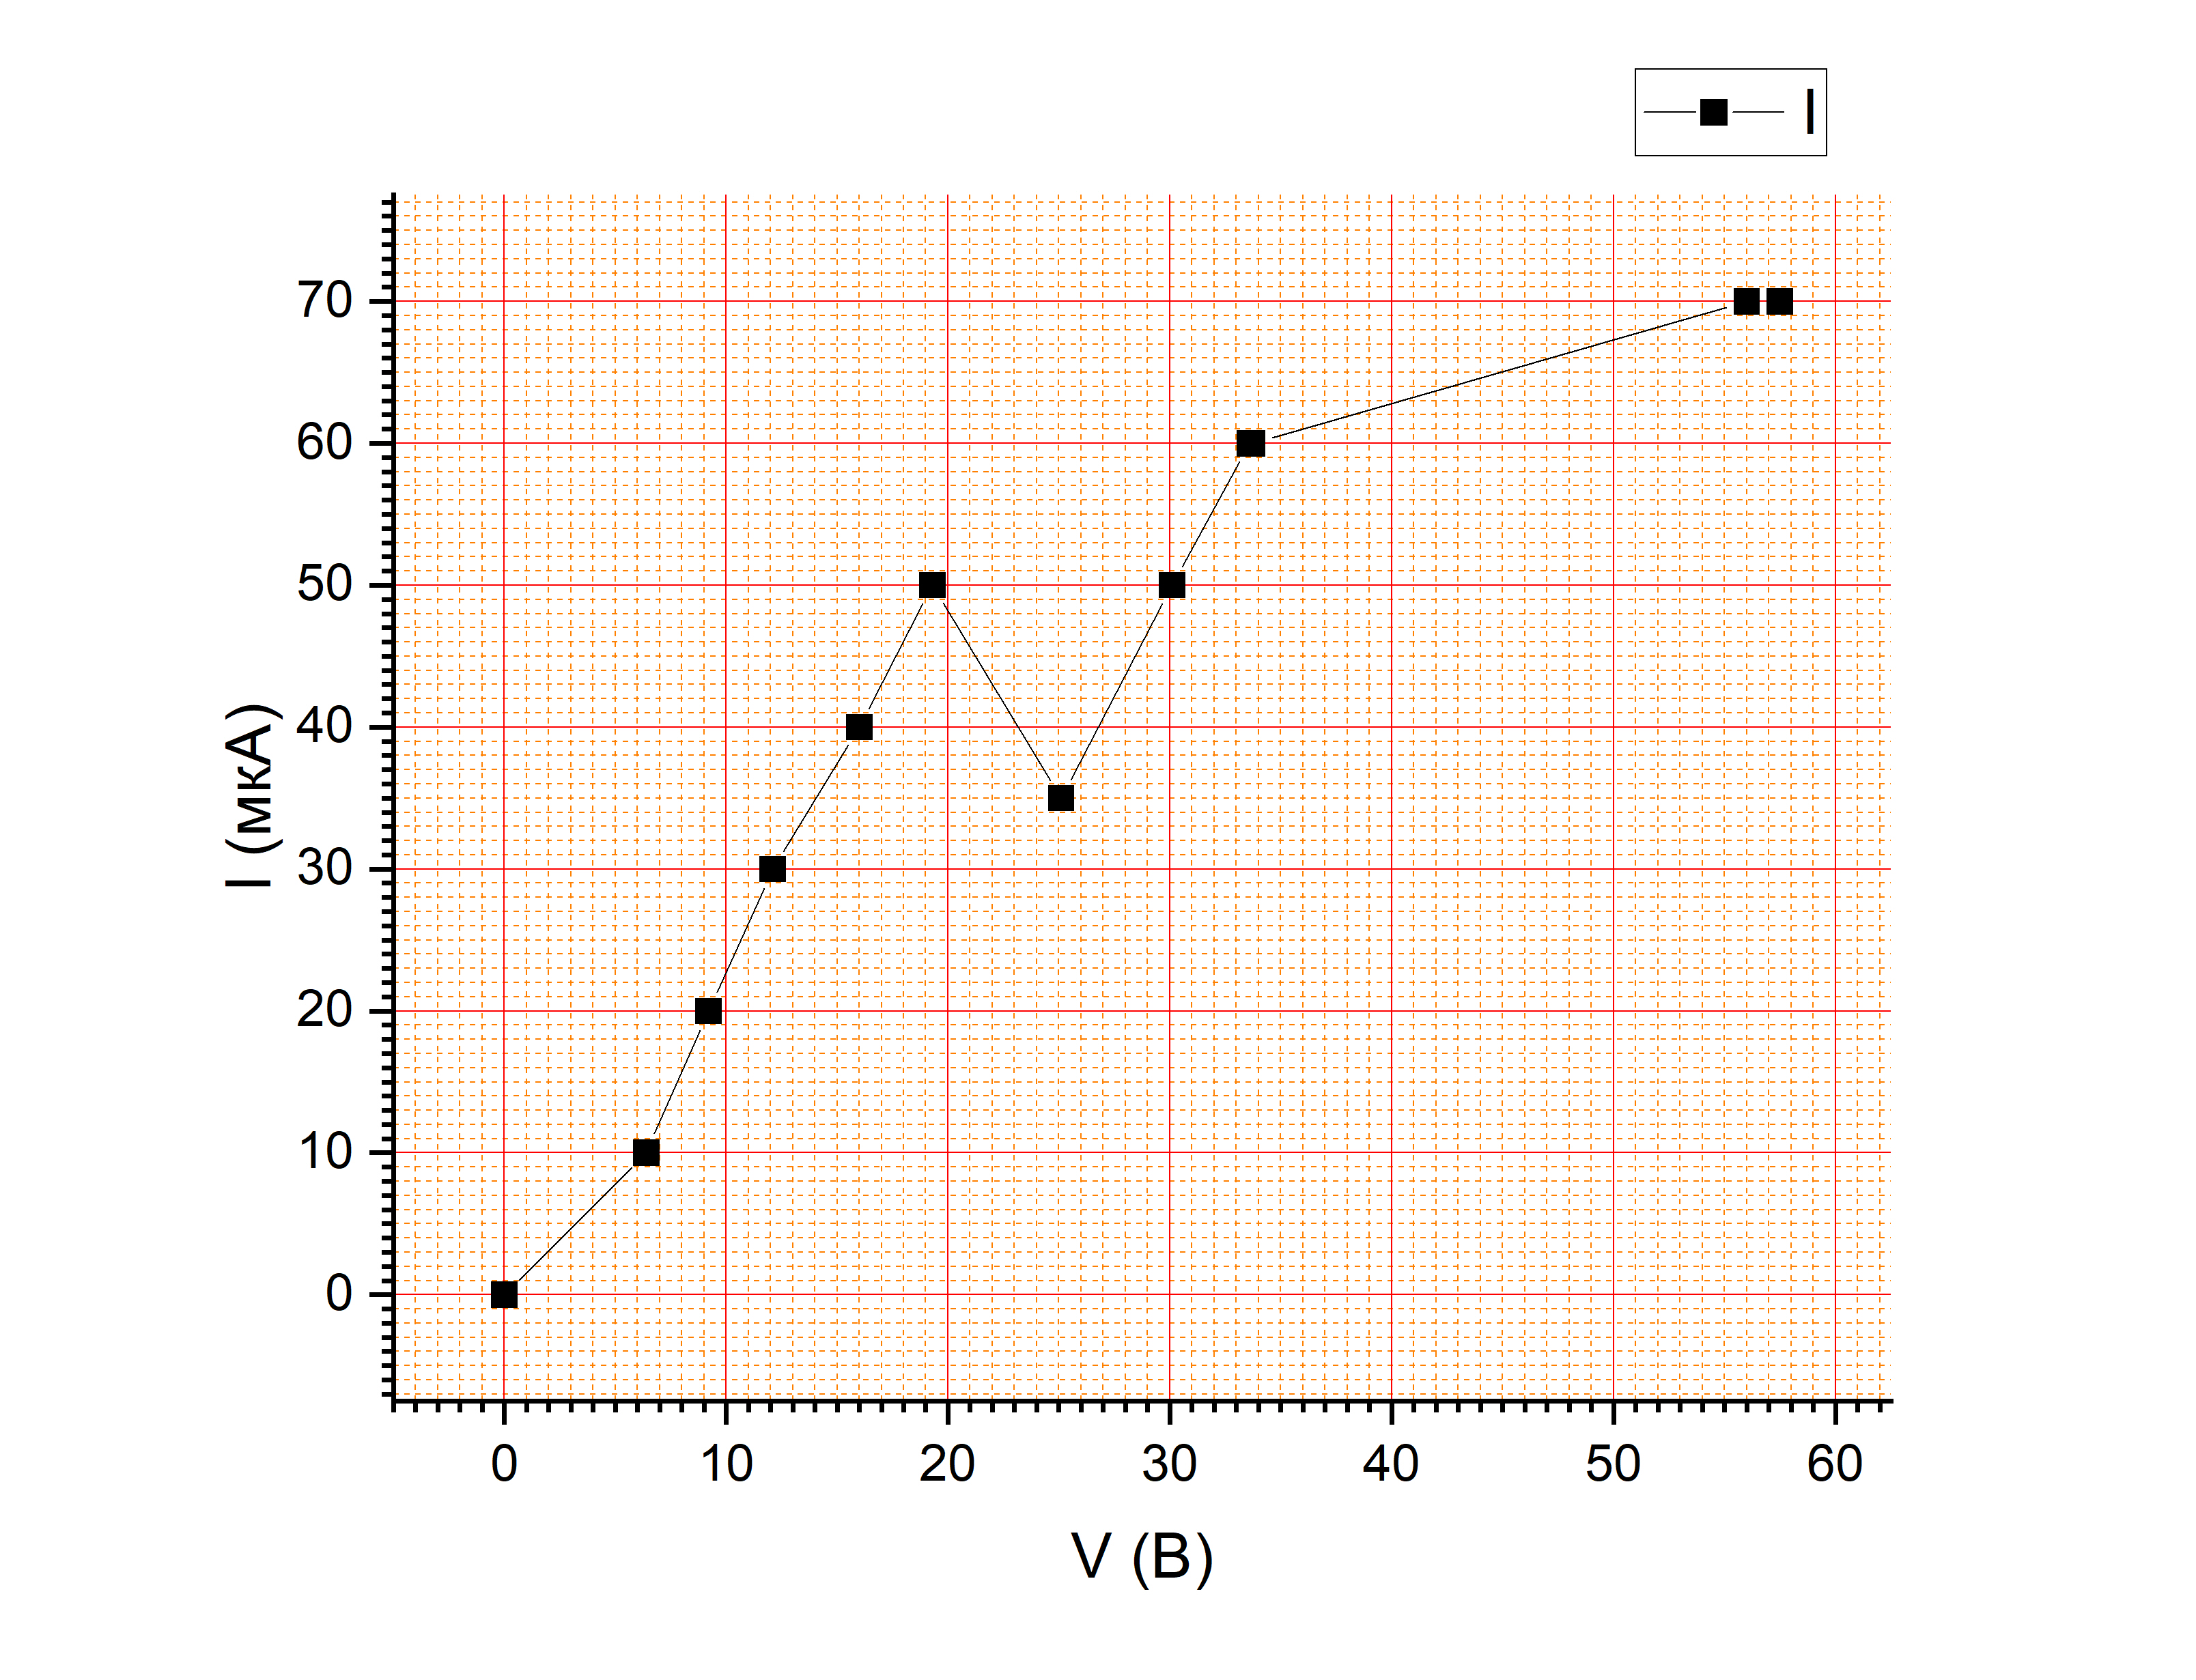
\includegraphics[width=0.7\linewidth]{Graph2}
	\caption{$V_з = 4 \;В$}
	\label{fig:graph2}
\end{figure}

\begin{figure}[tbh]
	\centering
	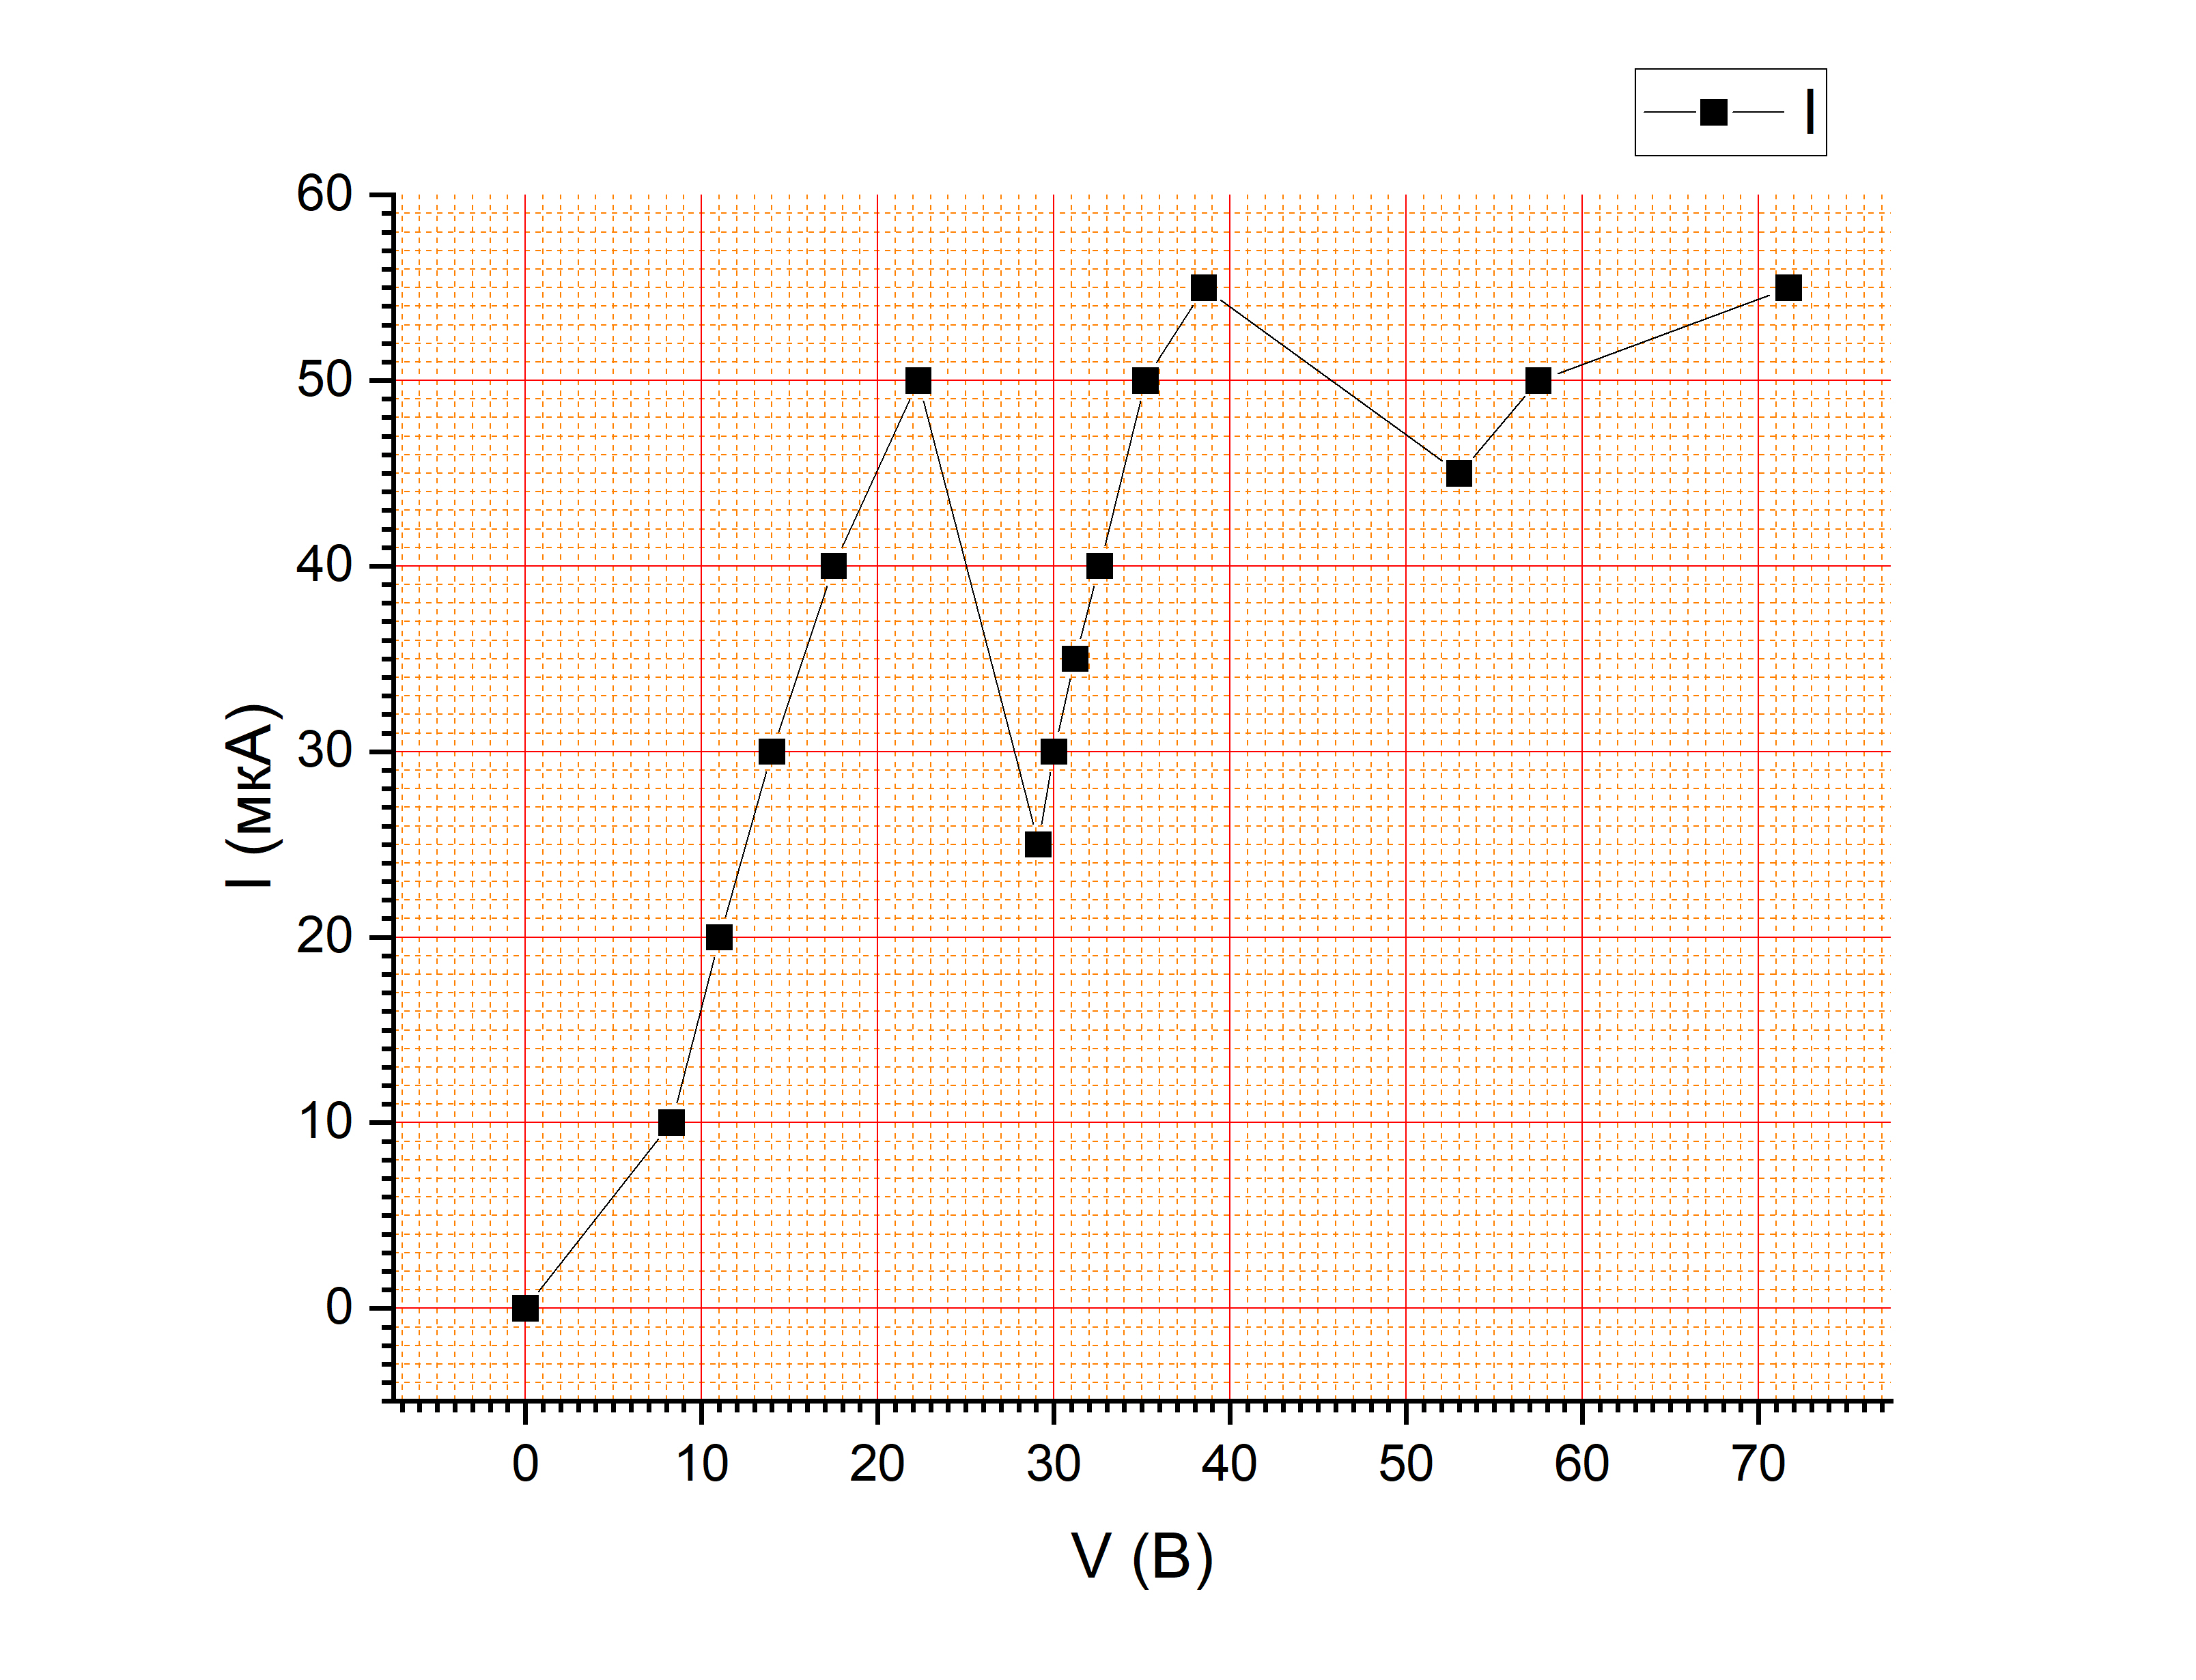
\includegraphics[width=0.7\linewidth]{Graph3}
	\caption{$V_з = 4 \;В$}
	\label{fig:graph3}
\end{figure}


\subsection{Оценка погрешностей}

В случае динамического метода, учитываются как случайные 
\begin{equation}\label{eq:погр}
	 \sigma = \sqrt{\frac{1}{N(N-1)}\sum (x-\left\langle x\right\rangle )^2},
\end{equation} 
так и систематические  погрешности $$ \delta = E \frac{\delta_{\Delta V}}{\Delta V}. $$

В статическом методе учёт инструментальных погрешностей не имеет смысла, т. к. случайные существенно больше. Используется формула \eqref{eq:погр}.

\section{Вывод}

Оба метода являются достаточно грубыми, однако статический даёт менее точный результат, т. к. необходимо заранее знать точку, в окрестности которой делать более качественные измерения. 

Референсное значение энергиии 1 уровня:
\begin{equation*}\label{key}
	E = 21.6 \;эВ.
\end{equation*}
В целом, в пределах погрешности, результаты согласуются с табличными.


\newpage

\begin{thebibliography}{9}
	\bibitem{Siv} Сивухин Д. В. \emph{Общий курс физики. Том 5 Атомная физика}, 2004
	\bibitem{max} \emph{Лабораторный практикум по общей физике. Квантовая физика} под ред. Ю. М. Ципенюка
\end{thebibliography}
\end{document}